  \section*{Instructions}
You will have \textbf{\testDuration} minutes to write code that should pass all
\textbf{\mycount} provided tests. \\
File in which all test are written is called \textbf{functions.test.js}.\\
The code for test is hashed, so You will not understand it’s details.\\

\begin{large}
	
	All tasks have to be implemented in this ONE and ONE ONLY file
	explicitly named \textbf{functions.js}. Any other name of file will
	not be accepted by automated checking server.
	
	After You will finish Yours implementation the
	\textbf{functions.js} have to be archived into the explicitly named
	\textbf{functions.zip} file, and this zip file have to be send onto
	the assignment.
	I do not accept any WORD or PDF or any other name or format.\\
	You have to create a file called \textbf{functions.js} and in this
	file create and export all functions/classes that are need by the
	tests, in given term:
\end{large}
\\
\begin{minted}{javascript}
module.exports = {}
module.exports.example = example
\end{minted}
Both of those files have to be inside same folder, Jest and NPM force this.\\

\section*{How to create env for testing}
All information was shown on laboratory.

\begin{enumerate}
	\item Create new empty folder,
	\item Download archive with \textbf{\textit{functions.test.js}} file from \textbf{MS
		Teams Assignment},
	\item Install library
	\textbf{\textit{\href{https://jestjs.io/docs/getting-started}{JEST}}}
	\begin{enumerate}
		\item Open terminal/command-prompt and go into prviously
		created empty folder, call \\ \textbf{npm install --save-dev jest}
		\item in \textit{package.json} add: \\
		\begin{minted}{javascript}
"scripts": {
	"test": "jest"
}
		\end{minted}
	\end{enumerate}
	\item To check if env was properly configured run: \\ \textbf{npm run test}
\end{enumerate}
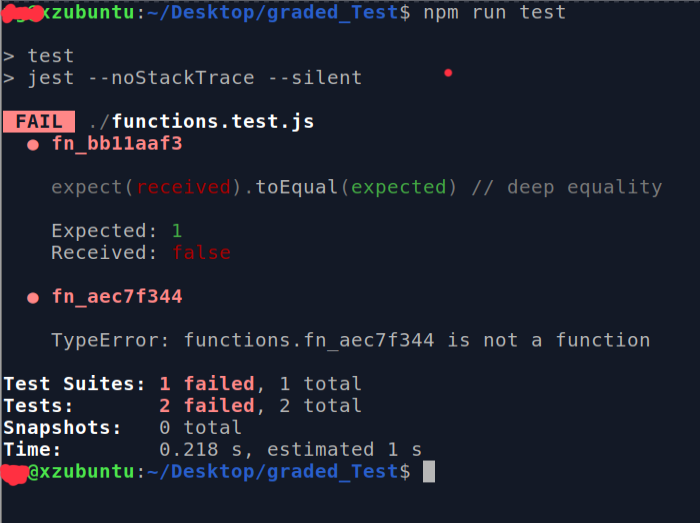
\includegraphics[width=\textwidth]{npm_run_test}
\subsection*{Compliance with the instructions}
File names and all other elements specified in the instructions must be exactly as required.
Otherwise, the tests will not be accepted.

\subsection*{Evaluation}
The evaluation covers only the files included in the resource. These files must not be modified by the reviewer.
Each test that passes gives 1 point, \textbf{provided that the program works correctly as a whole}.

\begin{remarkbox}[title=Working program]
	A working program is one that starts and finishes execution correctly, regardless of whether all tests pass.
	The program must not enter infinite loops or behave unexpectedly (e.g., cause critical errors or crashes) or return signals such as SIGTERM, SIGSEGV, SIGINT, SIGILL, SIGABRT, SIGFPE, etc.
\end{remarkbox}

\subsection*{Proof of operation}
Screenshots, console outputs, or other materials from your own runs do not constitute proof that the program works.
The code is executed by the reviewer, and only the test results are evaluated.

\subsection*{Resource guidelines}
You must submit your complete solution as a \textbf{zip} archive (\textit{project without the \textbf{node\_modules} folder}).
The archive name \textbf{must not} contain characters outside UTF-8 or special characters (including spaces, parentheses, etc.).
It is recommended that the archive name matches the name of the project provided in the resource.
Other archive formats (rar, tar.*, .7z, .dmg) will not be checked.

\subsection*{Project structure}
Before creating the archive, remove the \textbf{node\_modules} folder from your project.